\chapter{CountMax的算法设计与分析}
In this section, we describe the detailed implementation of CountMax, and analyze the traffic estimation error. CountMax mainly uses the lightweight design and cooperative deployment for a low computing overhead.


\section{Flow Recording}

To record flow traffic, similar to Count-Min, we maintain a bitmap with $w$ columns and $d$ rows, and a series of $d$ different hash functions $\{h_{1},...,h_{d}\}$. Each hash function $h_j$ maps any input (e.g., 5-tuple flow ID) to a random integer between $0$ and $w-1$:
\begin{equation}
\notag h_j: \{...\} \to \{0, ..., w-1\}
\end{equation}

Each slot in the bitmap has two fields: $Key$ and $Counter$. The bitmap and the set of hash functions form a sketch $S$. In the following sections we will discuss the parameters $d$ and $w$, and how they influence the performance of CountMax.%We should note that parameter $d$ will be explained later.


When the $i^{th}$ packet arrives at a switch, this switch first extracts its flow key, denoted as $f_i$. For every row $j$, we compute the hash value $u_{j}=h_{j}(f_i)$. If $Key_{j}[u_{j}]$ equals $f_i$, the corresponding counter field $Counter_{j}[u_{j}]$ increases by the size of the packet, denoted as $c_i$. Otherwise we compare $Counter_{j}[u_{j}]$ and $c_i$. If $Counter_{j}[u_{j}]$ is larger than $c_i$, $Counter_{j}[u_{j}]$ is decreased by $c_i$, i.e., $Counter_{j}[u_{j}] = Counter_{j}[u_{j}] - c_i$. Otherwise, we set $Counter_{j}[u_{j}]=c_i - Counter_{j}[u_{j}]$, and replace $Key_{j}[u_{j}]$ with $f_i$. The algorithm loops until all rows are updated. The details are shown in Alg. \ref{alg:count_max}.
%When a packet $p_i$ arrives at switch $v$, we first determine its flow key $f_i$. For every row, we compute the hash value $u=h(f_i)$, compare $Key[u]$ and $f_i$. If they equal, the corresponding field $Counter[u]$ increases by the traffic of $p_i$, denoted by $c_i$. Otherwise we compare $Counter[u]$ and $c_i$. If $Counter[u]$ is larger than $c_i$, $Counter[u_{j}]$ is decreased by $c_i$. Else we set $Counter[u]=c_i - Counter[u]$, and replace $Key[u]$ with $f_i$.
%\begin{equation}
%\notag count_x[k,h_x^k(i)] = count_x[k,h_x^k(i)]+c , \forall 1\le k \le d'_x
%\end{equation}

\begin{algorithm}
	\caption{CountMax's Updating for Each Arrival Packet}
	\label{alg:count_max}
	\begin{algorithmic}[1]
		\REQUIRE { $f_i$: flow key; $c_i$: packet size.}
		\FOR{every row $j$}
		\STATE {$u_j = h_{j}(f_i)$}
		\STATE {$f' = Key_{j}[u_j]$}
		\IF {$f_i = f'$}
		\STATE {$Counter_{j}[u_j] = Counter_{j}[u_j]+c_i$}
		\ELSE
		\IF{$Counter_{j}[u_j] > c_i$}
		\STATE{$Counter_{j}[u_j] = Counter_{j}[u_j]-c_i$}
		\ELSE
		\STATE{$Counter_{j}[u_j] = c_i-Counter_{j}[u_j]$}
		\STATE{$Key_{j}[u_j] = f$}
		\ENDIF
		\ENDIF
		\ENDFOR
	\end{algorithmic}
\end{algorithm}


%sending counter arrays to controller, which combines all arrays into one, queries made at the controller

\section{Flow Query}
%\input{query.tex}
For flow $f_i$, we query the counter in each row $j$ of sketch $S$ as follows:
\begin{equation}
\hat{a}_{i_{j}}=\left\{
\begin{aligned}
Counter_{j}[h_j(f_i)]&\text{, if $f_i=Key_{j}[h_j(f_i)]$}\\
0&\text{, otherwise}
\end{aligned}
\right.
\end{equation}

To derive the estimated flow size, we repeat the above query operations for all rows, and select the largest one, denoted as $\hat{a}_{i}$, as the estimation.
\begin{equation}
\label{eq:query}
\hat{a}_{i}=\max{\{\hat{a}_{i_{j}} , \forall j\}}
\end{equation}
%the last packet of a flow, flow size is collected in a packet-header field, and reported at the last switch to the controller

%use threshold to identify elephant flows.

\section{Analysis}
\label{subsec:analysis}
%\input{analysis.tex}

As discussed before, the CountMax sketch is able to identify large flows. Before analyzing its theoretical performance, we first give a definition of ``large flows" by introducing the Heavy Hitters problem.

Given a set of total $n$ flows with total traffic size $F$, and a parameter $\delta$ ($\delta \le 1$), the general Heavy Hitters problem is to identify flows whose traffic size is at least $\delta\cdot F$. In other words, if the traffic size of a flow is more than $\delta $ of the total traffic size in the network, this flows is called a $\delta$-``heavy hitter". Since Count-Min doesn't record flow keys, it cannot determine heavy hitter flows.


In this section, we will show that CountMax is a heuristic solution for Heavy Hitters and can derive an approximation result with bounded probability guarantee.

\begin{theorem}
	\label{tm:query}
	For every heavy hitter flow $f_i$ , $\hat{a}_i$ and $a_i$ are its estimated traffic size and the actual traffic size. Let $\tilde{d}$ denote the number of rows that flow $f_i$ occurs (i.e., $Key[h(f_i)] $ equals $f_i$) in the bitmap. We have the following inequality:
	\begin{equation}
	\label{eq:hhacc}
	Pr[1-\frac{e}{w\cdot \delta}\le \frac{\hat{a}_i}{a_i} \le 1] \ge 1-e^{-\tilde{d}}
	\end{equation}
\end{theorem}

\begin{proof}	
By Eq. \eqref{eq:query}, since $\hat{a}_i$ is always not larger than $a_i$, it follows $\hat{a}_i/{a_i} \le 1$. We define an indicator variable $I_{i,k,j}$ to denote whether hash collision of two flows $f_i$ and $f_k$ occurs on row $j $ or not. $I_{i,k,j}$ is 1 if ($f_i \ne f_k $ ) $\land $ ($h_j(f_i)=h_j(f_k)$), and 0 otherwise. That is, $I_{i,k,j}$ is 1 only when $h_j(f_i)$ and $h_j(f_k)$ equals, i.e. hash collision occurs. According to the pairwise independence of the hash functions, we have
\begin{equation}
E(I_{i,k,j})=Pr[h_j(f_i)=h_j(f_k)]\le \frac{1}{w}
\end{equation}
	

Similar to the analysis of Count-Min \cite{cormode2004improved}, we define variable $X_{i,j}=\sum\nolimits_{k=1}^{n}I_{i,k,j}\cdot a_k$ to denote the total traffic amount of flows colliding with flow $f_i$ in the $j^{th}$ row. Since the value of $Counter[h_j(i)]$ is ignored when $Key[h_j(f_i)]\ne f_i$, we need to find a sufficient condition to make $Key[h_j(f_i)]$ equals $f_t$. For any row $j$, if $a_i > X_{i,j}$, it means $a_i$ is more than half of total traffic processed by this slot. According to the pigeonhole principle, no matter the order of the arrival packets, $Key[h_j(f_i)]$ equals $f_i$. That means $\tilde{d}$ is at least the number of rows where $a_i > X_{i,j}$ is satisfied. From the pigeonhole principle we can also infer $Counter[h_j(i)]\ge a_i-X_{i,j}$. Besides, even if $a_i \le X_{i,j}$, since $Counter[h_j(i)]$ is at least zero, thus $Counter[h_j(i)]\ge a_i-X_{i,j}$ still holds. So, as long as $Key[h_j(f_i)] = f_i$, the following inequality holds.

\begin{equation}\label{eq:ai_xij}
Counter[h_j(i)]\ge a_i-X_{i,j}
\end{equation}

By the pairwise independence of $h_j$ and linearity of expectation, we have
\begin{equation}\label{eq:ex}\notag
E(X_{i,j})=E(\sum_{k=1}^{n}I_{i,k,j}\cdot a_k)\le\sum_{k=1}^{n} a_k\cdot E(I_{i,k,j})\le \frac{1}{w}\sum_{k=1}^{n}a_k.
\end{equation}

	
According to the definition of parameter $\delta$,
\begin{equation}\label{eq:ex-delta}
E(X_{i,j})\le \frac{1}{w}\sum_{k=1}^{n}a_k\le \frac{1}{w}\cdot \frac{a_i}{\delta}
\end{equation}

	
Similar to the analysis for Count-Min\cite{cormode2004improved}, we have following derivation. For simplicity, $\forall j$ means $\forall j\in \{j|Key[h_j(f_i)] = f_i\}$.
\begin{align}\notag
&Pr[\hat{a}_i< a_i-\frac{e}{w}\cdot\frac{a_i}{\delta}]\\\notag
&=Pr[\forall j, Counter[h_j(f_i)]<a_i-\frac{e}{w}\cdot\frac{a_i}{\delta} ]\\\notag
&\le Pr[\forall j, a_i-X_{i,j} <a_i-\frac{e}{w}\cdot\frac{a_i}{\delta} ] \text{ (Eq. \eqref{eq:ai_xij})}\\\notag
&=Pr[\forall j, X_{i,j} > \frac{e}{w}\cdot\frac{a_i}{\delta} ]\\\notag
&\le Pr[\forall j, X_{i,j}>e\cdot E(X_{i,j})]\text{ (Markov inequality)}\\\notag
&<e^{-\tilde{d}}
\end{align}
	
As a result, it follows:
\begin{equation}
Pr[\frac{\hat{a}_i}{a_i} \ge 1-\frac{e}{w\cdot \delta}]\ge 1-e^{-\tilde{d}}
\end{equation}
\end{proof}


Next we analyze the expectation of variable $\tilde{d}$.

\begin{theorem}\label{tm:acc}
For any query of a heavy hitter, $E[\tilde{d}]\ge d\cdot(1-\frac{1}{w\cdot\delta})$.
\end{theorem}

\begin{proof}
Consider flow $f_i$ and row $j$, we prove that the probability of $Key[h_j(f_i)] = f_i$ is at least $1 - \frac{1}{w\cdot\delta}$. If the traffic amount of flow $f_i$ is larger than 1/2 of total amount of flows that hashed to the slot $h_j(f_i) $, or we say $a_i > X_{i,j}$, it is obvious that $Key[h(f_i)] $ equals $f_i$.

	By the Markov inequality and Eq. \eqref{eq:ex-delta},
	\begin{align}\notag
	Pr[X_{i,j}>a_i] &\le \frac{E[X_{i,j}]}{a_i}\\\notag
	&\le \frac{1}{w}\cdot\frac{a_i}{\delta}\cdot\frac{1}{a_i}\\
	&\le \frac{1}{w\cdot\delta}
	\end{align}
	Thus $Pr[Key[h_j(f_i)]=f_i]\ge 1- Pr[X_{i,j}>a_i] \ge 1-\frac{1}{w\cdot\delta}$. Obviously $E[\tilde{d}]$ is no less than the count of rows that meet $Key[h_j(f_i)]=f_i$. Since every row is individual, we have $E[\tilde{d}]\ge d\cdot(1-\frac{1}{w\cdot\delta})$.
\end{proof}

Besides, since the hash operation costs $O(1)$ time and runs once for each row, we can easily conclude that:
\begin{theorem}\label{tm:time}
CountMax needs $O(d)$ update operations for each arrival packet, where $d$ is the number of rows in the CountMax.
\end{theorem}


\begin{figure}[!h]
	\centering
	\begin{minipage}[t]{0.48\linewidth}		
		%\begin{figure}[!t]
		\centering
		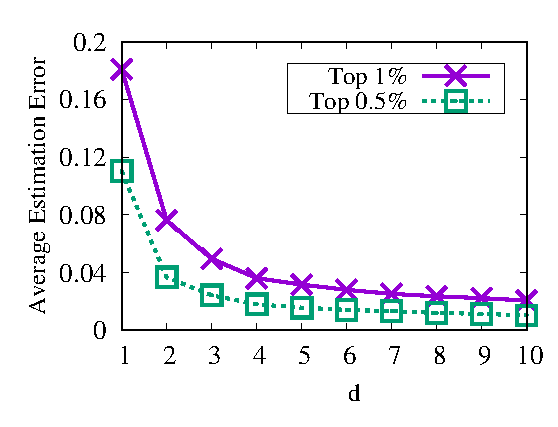
\includegraphics[width=\linewidth]{fig/cm_d_err.eps}
		\caption{Estimation Error vs $d$}
		\label{fig:cm,d,acc}
		%\end{figure}
	\end{minipage}\vspace{-0.6em}
\hspace{0.4em}
	\begin{minipage}[t]{0.48\linewidth}
		\centering
		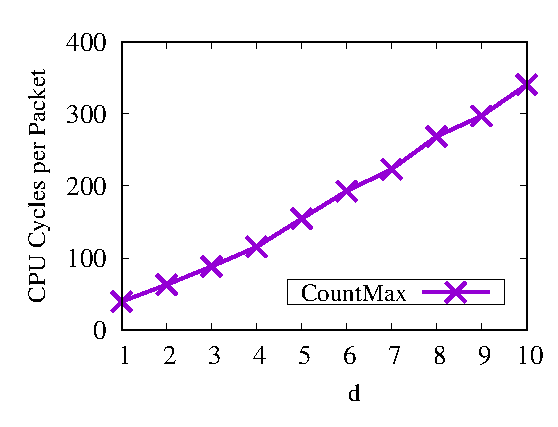
\includegraphics[width=\linewidth]{fig/cm_d_cpu.eps}
		\caption{Average CPU cycle of updating}
		\label{fig:cm,d,cpu}
	\end{minipage}\vspace{-0.6em}
\hspace{0.1em}
\end{figure}


\section{Cooperative CountMax}\label{subsec:distributedimplementation}


We introduce how to implement the cooperative deployment of CountMax to further reduce the computing overhead on switches. There are two different ways to reduce the computing overhead on each switch.


One is to reduce the number of rows of CountMax. From Fig. \ref{fig:cm,d,acc}, with more rows in a CountMax sketch, the average estimation error becomes smaller. However, the decreasing ratio becomes smaller as $d$ grows. For example, the average estimation error with $d=3$ is similar to that with $d=10$. Even with $d=2$, the average estimation error is only about 5\%. On the contrary, Fig. \ref{fig:cm,d,cpu} shows that the computing overhead of CountMax is linearly increasing with the number of rows (i.e., $d$).


\begin{figure}[h]
   \centering
   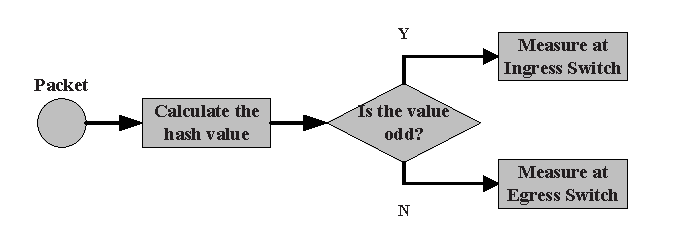
\includegraphics[width=\linewidth]{fig/filter_measure.eps}
   \caption{Illustration of the Cooperative Measurement Framework}
   \label{fig:filtermeasurement}
\end{figure}


The other way is to reduce the amount of processed traffic through cooperation, e.g., cSamp \cite{sekar2008csamp}. To measure traffic of flows, a natural way is to build an individual and centralized module of CountMax on each switch. As a result, this sketch will measure all packets through this switch. In this paper, we use a simple way for cooperative traffic measurement among ingress switches and egress switches. The traffic processing procedure is illustrated in Fig. \ref{fig:filtermeasurement}. When a packet arrives at an ingress switch, it uses a common hash function to generate an integer for this packet using its 5-tuple information. If this is an odd number, the ingress switch will measure this flow. Otherwise, this packet will be measured by the egress switch.

We analyze the estimation error of cooperative CountMax in a simple network. Without loss of generality, suppose that there is only two switches in the network. One is the ingress switch, and the other is the egress switch. Assume that the total traffic amount from the ingress switch to the egress switch is $F$. The ingress switch processes the traffic ratio $\gamma_1 $, and the amount of processed traffic is $F_1 =\gamma_1\cdot F $. Meanwhile, the egress switch processes the traffic ratio $\gamma_2 $, and the amount of processed traffic is $F_2 =\gamma_2 \cdot F $. Obviously, $\gamma_1 + \gamma_2 = 1$. 

%\begin{equation}\label{eq:coop_f}
%\left\{
%\begin{aligned}
%F_1&=\gamma_1\cdot F\\
%F_2&=\gamma_2\cdot F
%\end{aligned}
%\right.
%\end{equation}

Now we focus on the ingress switch. Let $f$ denotes a $\delta$-heavy hitter of the entire flow set. It means that the traffic size of $f$ is larger than $\delta \cdot F$. If $f$ is measured by the ingress switch, %by Eq. \eqref{eq:coop_f},
 $f$ is actually a $\delta/\gamma_1$-heavy hitter of flows measured by the ingress switch. According to Theorem \ref{tm:query} and Theorem \ref{tm:acc}, the estimation of a $\delta$-heavy hitter in the cooperative CountMax holds following inequalities:

\begin{equation}\label{eq:coop_acc}
\left\{
\begin{aligned}
&Pr[1-\frac{e\cdot \gamma_x}{w\cdot \delta}\le \frac{\hat{a}_i}{a_i} \le 1] \ge 1-e^{-\tilde{d}}\\
&E[\tilde{d}]\ge d\cdot(1-\frac{\gamma_x}{w\cdot\delta})
\end{aligned}
\right.
\end{equation}

$\gamma_x$ denotes $\gamma_1$ or $\gamma_2$, depending on the flow is measured by ingress/egress switches. We can define $\gamma_m = \max \{\gamma_1, \gamma_2\}$ to give a lower bound for error estimation. Under the best situation, $\gamma_1=\gamma_2=1/2$. In practice, $\gamma_1$ and $\gamma_2$ are usually close to each other. According to Eq. \eqref{eq:coop_acc}, the cooperative CountMax method narrows the range of $\frac{\hat{a}_i}{a_i}$ and $E[\tilde{d}]$ by ratio $\gamma_m $.


%In practical situations, switch $v$ may be the ingress switch of some flows and the egress switch of other flows at the same time. If every switch has balanced ingress/egress flows, this cooperative method doesn't improve a lot. However, in realistic network, there are many hosts that mainly send data but seldom receive data, or vice versa. Thus our cooperative method can help balancing the computing overhead between switches.




%A natural way is to build an individual and centralized module of CountMax on each switch. As discussed above, the computing overhead is important for sketch design. To ensure the estimation accuracy, we may choose a feasible value (e.g., 6-7) for $d$, and the CPU resource cost for each update operation grows. Due to the disadvantage of centralized design, we present a cooperative manner for CountMax. Now we give an example to illustrate the cooperative CountMax in a structured topology, e.g., Fat-tree \cite{al2008scalable}, in which switches are classified into core, aggregation, and edge levels. All switches are divided into two categories, non-egress switches and egress switches. In each non-egress switch, there deploys a sketch-based filter so as to filter those mice flows. In the egress switch, we will deploy a CountMax sketch.





%\begin{figure}[!t]
%	\centering
%	\begin{minipage}[t]{0.48\linewidth}		
%		%\begin{figure}[!t]
%		\centering
%		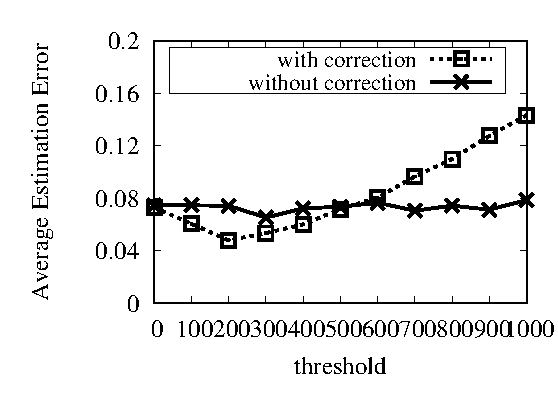
\includegraphics[width=\linewidth]{fig/ths_appr.eps}
%		\caption{Estimation Error vs threshold}
%		\label{fig:cm,ths,acc}
%		%\end{figure}
%	\end{minipage}\vspace{-0.6em}
%	\hspace{0.4em}
%	\begin{minipage}[t]{0.48\linewidth}
%		\centering
%		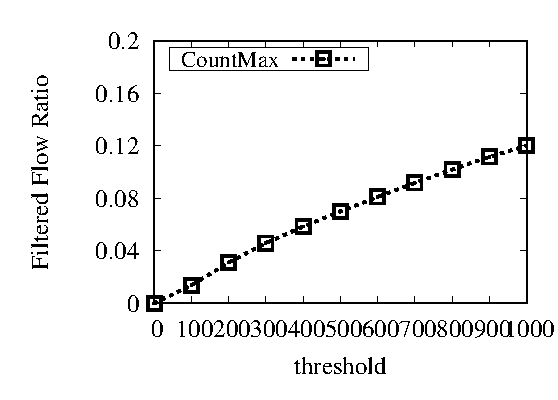
\includegraphics[width=\linewidth]{fig/ths_filter.eps}
%		\caption{Filtered Flow Ratio vs threshold}
%		\label{fig:cm,ths,flow}
%	\end{minipage}\vspace{-0.6em}
%	\hspace{0.1em}
%\end{figure}





%an ingress switch, this switch will generate a hash value $\omega $, with $0 \le \omega \le 1 $, using its 5-tuple information, and add $\omega $ %with the ingress-switch ID
% to the packet header. Moreover, we maintain a state bit on each packet, initially as 0, which denotes this packet has not been measured. The real-time packet processing framework is illustrated in Fig. \ref{fig:filtermeasurement}. Specifically, when a packet arrives at a switch $v_i$, including its ingress switch, there are two cases:
%\begin{enumerate}
%\item If the state bit of a packet is 0, it has not been measured. There are two sub-cases.
%\begin{enumerate}
%\item If $\omega $ is less than or equal to its weight $\omega_i $ or it is the egress switch of this packet, switch $v_i $ will measure this packet, and set the state bit to 1.
%\item Otherwise, the switch updates the variable as $\omega = \omega - \omega_i $ in the packet header.
%\end{enumerate}
%\item If the state bit is 1, it is no need to measure this packet. %this packet will not be measured on this switch. %the switch just forwards this packet to the next-hop switch according to the matching rule.
%\end{enumerate}




%We first take a simple test to observe the impact of parameter $d$ on different performance metrics (e.g., estimation error and computing overhead) on Windows 10 OS with Intel Core i5-6500 CPU. In the test, all flows follow the same distribution as described in Section \ref{sec:evaluation} and we calculate the top 1\% flows. Fig. \ref{fig:cm,d,acc} shows the relationship between the estimation error and $d$. We find that as $d$ increases, both the estimation error and its slope decrease. Fig. \ref{fig:cm,d,cpu} shows that the computing overhead is a linear function of $d$, which confirms Theorem \ref{tm:time}.



%Distributing a uniform number of rows on each switch is a simple implementation solution. We can also design flexible sketch deployment for different topologies and applications. For example, in a Fat-tree topology \cite{al2008scalable}, switches are classified into core, aggregation, and edge levels. Since core switches process a large amount of flows, their statistics may be with less accuracy, and make a little contribution to a query. To be flexible, we deploy $2 $ rows on each edge switch, $1 $ row on each aggregation switch, so that every flow (through two edge switches and one aggregation switch) will be monitored by at least $5 $ rows. This solution also reduces the memory usage compared with the previous uniform distribution setting. Assume that the Fat-tree topology has $80$ switches (including 16 cores, 32 aggregations, and 32 edges). The flexible deployment requires total $32 \times 1 + 32\times 2 = 96$ rows, while the fixed-row distributed deployment solution requires $80 \times 2 = 160$ rows. Thus, we reduce the total memory cost by 40\% and eliminate the computing overhead of core switches while the estimation accuracy only decreases no more than 10\% by Fig. \ref{fig:cm,d,acc}.



\section{Application of CountMax}\label{subsec:flowrerouting}
%\input{application.tex}
In this section, we discuss an application of CountMax, namely flow rerouting.

%\section{Flow Rerouting}

Flow rerouting is necessary and important for many practical applications, e.g., link load balancing and bypassing broken link\cite{xu2017incremental}. For these applications, statistics of those large flows are much more valuable \cite{xu2017scalable}. The controller monitors the link (or port) traffic load by periodically collecting the port statistics information from switches. When the controller detects that some links are overloaded, flow rerouting is required. To this end, the controller collects the sketch information from switches, identifies those elephant flows, denoted by $\Gamma^e$. Since elephant flows consist of most traffic in the network, we can optimize the link utilization by rerouting these flows using different rerouting algorithms. For example, we can use a simple greedy method. First we rank all these elephant flows in the decreasing order of traffic size. For each flow $\gamma \in \Gamma^e$, the controller finds the least congested path between the flow's endpoints as its new route. After determining new routes for all the elephant flows in $\Gamma^e$, we execute the route reconfiguration \cite{jin2014dynamic} \cite{xu2017joint}. Since we only reroute elephant flows and the number of elephant flows is much smaller than the total number of flow, the route reconfiguration delay is reduced. Since CountMax is a compact data structure, and the number of ports on each switch is usually small (e.g., 24 or 48), collecting sketch and port statistics information from all switches will not bring significant overhead on the controller.



%\section{CountMax-Based Hierarchical Heavy Hitters (HHH)}

%If a flow $f$ has destination host of IP address 10.11.12.13, it has different keys in different levels. For the 1st level the key of $f$ is 10.0.0.0, for the 2nd level it's 10.11.0.0, and so on.

%As an extension of Heavy Hitters, Hierarchical Heavy Hitters (HHH) is to find out the heavy hitters in different levels of a hierarchical model. For example, we can classify flows according to subnets of the destination host, and there can be multi levels of subnets. More specificity, suppose there are 4 levels, denoted by level 0 to level 3, and the subnet mask is 255.255.255.255 for level 0, 255.255.255.0 for level 2, and so on. For level 0, it directly deals with flows; For higher levels, they deal with sets of flows, according to the subnets that flows belong to. Given a threshold $\delta$, for level 0, the hierarchical heavy hitters are just the heavy hitter flows. For the $i$th level ($i>0$), it's a bit more complex.

%As mentioned before, the higher levels deal with flow sets instead of flows. For the $i$th level ($i>0$), the weight of a flow set $s$ is defined as the sum of traffic of flows, where each flow satisfies: the flow belongs to $s$, but does not belong to any HHH of lower levels.

%Authors of \cite{cheung2006finding} have discussed the implementation of general HHH based on Count-Min. However, Count-Min cannot find out HHH flows since it doesn't record flow keys. Suppose that there are $g$ levels of hierarchies. To solve the HHH problem, we need to keep $g$ CountMax sketches, denoted by $C_1, ... ,C_g$, where $C_i$ corresponds the $i$th hierarchical level from top to bottom.

%When a packet arrives, for every level $i \in \{1, ..., g\}$, we first calculate the level-specified key $key_{i}$. In the previous example, if a flow $f$ has destination host of IP address 10.11.12.13, its $key_0$ is 10.11.12.13, $key_1$ is 10.11.12.0, $key_2$ is 10.11.0.0, and $key_3$ is 10.0.0.0. Then we update $C_{i}$ using $key_{i}$ as the key. To find out heavy hitters of every hierarchy level, we just iterate the CountMax sketches from $C_g$ to $C_1$, and figure out the result according to the definition of HHH.

